\section{Meilenstein 5: 07.08.2019 - 04.09.2019}
Der fünfte Meilenstein ist der letzte der Implementierungsphase.
Mit Abschluss des Meilensteins gilt für die Projektgruppe ein Feature Freeze.
In diesem Meilenstein wird das Ziel verfolgt, das Gesamtsystem mit gezielten Features abzurunden und fertigzustellen.
Durch die bereits bestehenden Schnittstellen zwischen den einzelnen Komponenten konnte vor allem im Frontend der Fokus auf neue Features gelegt werden.
Im UIS"=Frontend sollte insbesondere die Performanz verbessert sowie eine Export"=Funktion für die Sensorknotendaten bereitgestellt werden.
Weiterhin sollen in der Navigationsapplikation die gleiche Heatmap angezeigt werden, die auch im UIS genutzt wird.
Ein weiteres sehr zentrales Feature, welches im vierten Meilenstein implementiert wird, ist das dynamische Routing.
Vom Nutzer kann bei der Routenplanung ein entsprechendes Intervall eingestellt werden, in dem die Umweltparameter überprüft werden, im bei signifikanten Änderungen eine neue Route für den Nutzer zu berechnen.
Zudem sollen weitere Features, wie das Routing nach anderen Umweltparametern und das Anzeigen von Informationen beim Routing im vierten Meilenstein fertiggestellt werden.


Ein weiteres zentrales Feature ist die Sensorknotenverwaltung, die als Single"=Page"=Webseite implementiert wird.
Hier soll es möglich sein, neue Sensorknoten in der IoT"=Plattform anzulegen und verändern zu können.
Neben der Sensorknotenverwaltung werden in der IoT"=Plattform aufbereitete PM25"=Werte bereitgestellt, welche die Luftfeuchte berücksichtigen.
Diese Werte können für jeden Sensorknoten in den Zeitreihen des UIS"=Frontends angezeigt werden.


Im Kontext der Sensorknotenfirmware wird das Installationstool für Sensorknotenbetreiber bereitgestellt, sodass diese den Sensorknoten auf einfache Weise flashen und konfigurieren können.
Außerdem wird die Möglichkeit geschaffen, die Sensorknoten automatisch zu updaten.
Die virtuellen Sensorknoten sollen neben der Mock"=Strategie und der Random"=Strategie zukünftig auch eine Gewichtungsstragie verfolgen können.
In diesem Zusammenhang soll die Möglichkeit geschaffen werden, diverse reale Sensorknoten anzugeben, die in der Berechnung des virtuellen PM25"=Wertes berücksichtigt werden, sodass ein möglichst realistischer Wert für den virtuellen Sensorknoten erzeugt wird.

\begin{figure}[!htb]
	\centering
	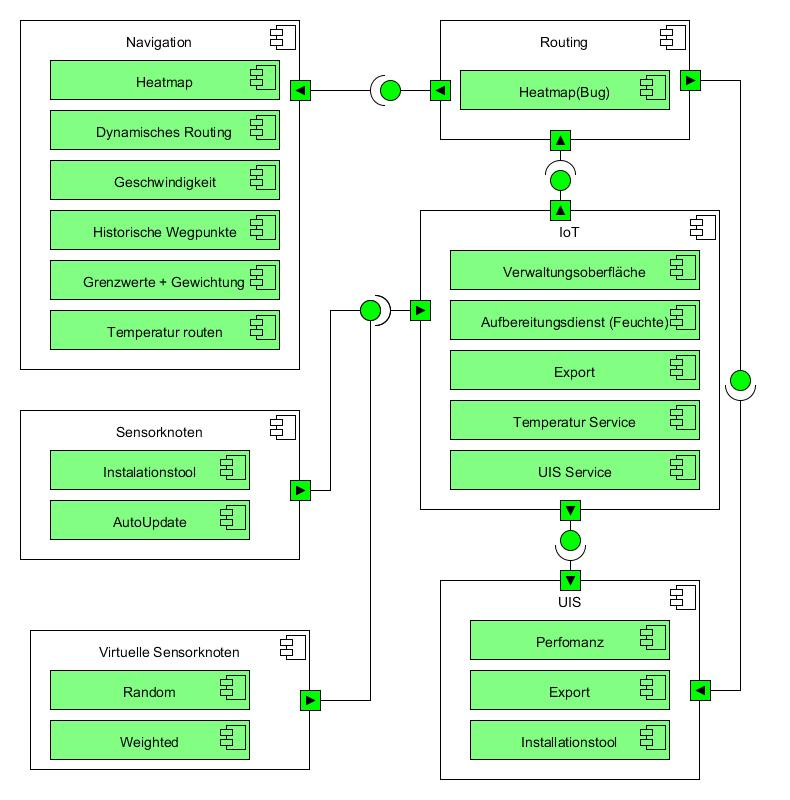
\includegraphics[width=\textwidth]{./ressourcen/bigpicture4.png}
	\caption{Big Picture des fünften Meilensteins}
	\label{fig:bigpicture4}
\end{figure}

In \Fig{bigpicture4} zeigt sich abschließend, dass alle geplanten Ziele für den fünften Meilenstein erreicht wurden.
Durch die Fertigstellung der Schnittstellen zwischen den einzelnen System wird das Arbeiten an Features weniger Komplex.
Hinzu kommt die zunehmende Erfahrung der Projektgruppe in ihren Bereichen, sodass die Umsetzung einer funktionalen Anforderung zum Teil wesentlich schneller voran geht, als am Anfang der Implementierungsphase.
Abschließend wird mit dem fünften Meilenstein das System erfolgreich abgerundet.
Durch das Erreichen aller Ziele, kann in der letzten Phase des Projektes der Fokus auf die Qualität des Systems gelegt werden, welche schon während des Projektes durch Dinge wie die Definition of Done und Ähnliches berücksichtigt wurde.
Dem gegenüber stehen Dinge wie die User Tests, um beispielsweise Feedback einzuholen.
Daher wird für den letzten Monat der Fokus der Projektgruppe auf das Testen, Bugfixing und Dokumentieren gelegt.